\documentclass{article}%
\usepackage[T1]{fontenc}%
\usepackage[utf8]{inputenc}%
\usepackage{lmodern}%
\usepackage{textcomp}%
\usepackage{lastpage}%
\usepackage[head=40pt,margin=0.5in,bottom=0.6in]{geometry}%
\usepackage{graphicx}%
%
\title{\textbf{Denuncian que efectivos de las Faes asesinaron a dos polichacao}}%
\author{Diario El Universal}%
\date{07/03/2019}%
%
\begin{document}%
\normalsize%
\maketitle%
\textbf{URL: }%
http://www.eluniversal.com/sucesos/34977/denuncian{-}que{-}agentes{-}de{-}las{-}faes{-}asesinaron{-}a{-}dos{-}polichacao\newline%
%
\textbf{Periodico: }%
EU, %
ID: %
34977, %
Seccion: %
sucesos\newline%
%
\textbf{Palabras Claves: }%
NO\_TIENE\newline%
%
\textbf{Derecho: }%
2.1%
, Otros Derechos: %
\newline%
%
\textbf{\textit{El alcalde Gustavo Duque exigió justicia ante este hecho.Las víctimas fueron Alexander Eligio Duarte (Polichacao activo) y Fernando Lira, exfuncionario de este organismo policial.}}%
\newline%
\newline%
%
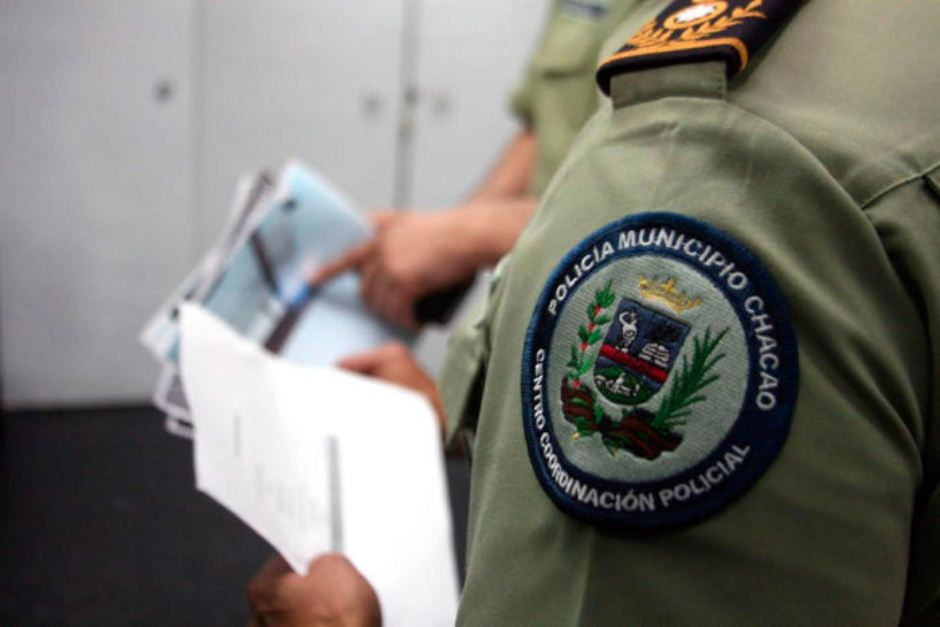
\includegraphics[width=300px]{EU_34977.jpg}%
\newline%
%
Dos funcionarios de Policía de Chacao (Polichacao), uno activo y otro retirado, fueron asesinados ayer en horas~ de la tarde presuntamente en manos de oficiales de las Fuerzas de Acciones Especiales (Faes) de la Policía Nacional en un hecho registrado en Guarenas la denuncia la confirmó el alcalde de Chacao, Gustavo Duque a través de su cuenta en twitter.%
\newline%
%
Según el informe policial de las Faes, Alexander Eligio Duarte y Fernando Lira fueron ultimados durante un "enfrentamiento armado para la liberación de un cautivo".%
\newline%
%
Sin embargo, el alcalde de Chacao exigió que se investigue este hecho.%
\newline%
%
\end{document}